\documentclass[11pt]{article}
\usepackage{array, url, kantlipsum, listings, xcolor}
\usepackage[margin=1in]{geometry}
\usepackage{graphicx, float, courier}
\usepackage[section]{placeins}
\usepackage[utf8]{inputenc}
\graphicspath{ {output/} }

\lstdefinestyle{terminal}
{
    backgroundcolor=\color{white},
    basicstyle=\footnotesize\color{black}\ttfamily,
    frame=tb,
    numbers=left
}
\makeatletter
\long\def\@makecaption#1#2{%
	\vskip\abovecaptionskip
		\bfseries #1: #2\par
	\vskip\belowcaptionskip}%
\makeatother

\title{Assignment 4 \\CPSC 526 Fall 2017 \\ November 12, 2017}
\author{
\begin{tabular}{c c}
Mason Lieu & Shane Sims\tabularnewline
ID: 10110089 & ID: 00300601\tabularnewline
Tutorial 04 & Tutorial 04 \tabularnewline
\url{mlieu@ucalgary.ca} & \url{shane.sims@ucalgary.ca}
\end{tabular}}
\date{}

\begin{document}
\maketitle

\section*{How to run Server and Client}
\begin{lstlisting}[style=terminal, title={Running the server}]
python FTserver.py <port number> <key>
\end{lstlisting}
\begin{lstlisting}[style=terminal, title={Running the client}]
python FTclient.py <command> <file name> <host>:<port> <cipher> <key> 
\end{lstlisting}

\section*{AES256 upload/download/checksum test}

	\begin{figure}[H]
	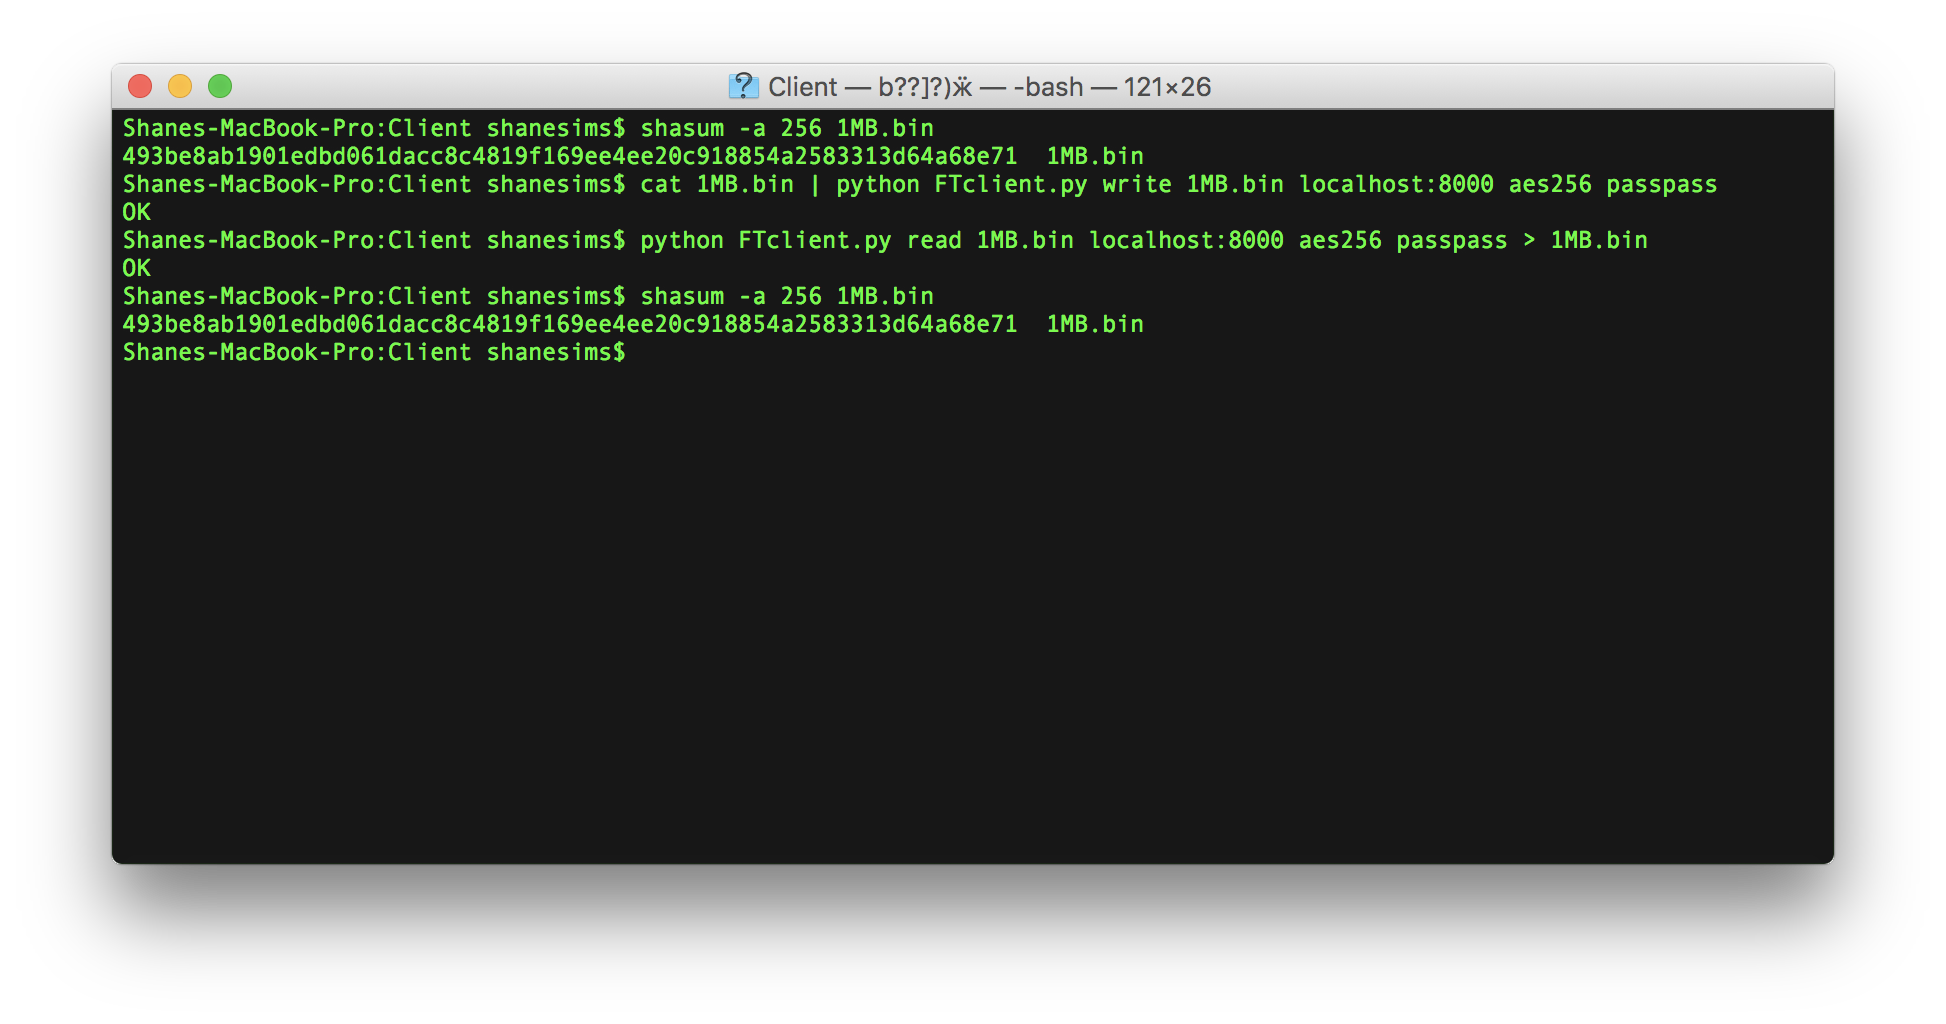
\includegraphics[scale=0.5, trim={0cm 0cm 0cm 0cm}, clip]{test}
	\caption{Test for correctness}
	\end{figure}

\section*{Communication Protocol}
\subsection*{\texttt{write} command}
\begin{center}
\begin{tabular}{ |c|c|c| } 
 \hline
 ~& Client & Server\\
 \hline\hline
 1. & send \texttt{write} & ~ \\ 
 \hline
 2. & ~ & send {ACK} \\ 
 \hline
 3. & send \texttt{fileName} & ~ \\ 
 \hline
 4. & ~ & echo \texttt{fileName}\\
 \hline
 5. & encrypt 1024 byte blocks and \texttt{send} & ~\\
 \hline
 6. & ~& \texttt{receive} and decrypt blocks\\
 \hline
 7. &\texttt{send} EOF &~\\
 \hline
 8. & ~& \texttt{send} status/result flag\\
 \hline
 9. & \texttt{print} status & ~\\
 \hline
\end{tabular}
\end{center}

\subsection*{\texttt{read} command}
\begin{center}
\begin{tabular}{ |c|c|c| } 
 \hline
 ~& Client & Server\\
 \hline\hline
 1. & \texttt{send} \texttt{read} & ~ \\ 
 \hline
 2. & ~ & \texttt{send} {ACK} \\ 
 \hline
 3. & \texttt{send} file name & ~ \\ 
 \hline
 4. & ~ & \texttt{send} file size\\
 \hline
 5. & ~& encrypt 1024 byte blocks and \texttt{send}\\
 \hline
 6. & \texttt{receive} and decrypt blocks &~\\
 \hline
 8. & \texttt{send} status/result flag &~\\
 \hline
 9. & \texttt{print} status & ~\\
 \hline
\end{tabular}
\end{center}


\section*{Timing Tests}



\end{document}

